\section{Summarization Framework}
\label{sec:algorithm}

The major motivation of our work is to find a concise and intuitive summarization of a given research topic. More concretely, we want to select a set of representative terms that best describe the hot spots and major achievements along the development of the research topic, meanwhile, capture the temporal evolutionary pattern within the research area. We formulated the problem as a graph partitioning task. At a high level, the proposed summarization framework consists of three stages.

\begin{itemize}
    \item {\bf Document retrieval.} First, given a research topic $q$ needs to be summarized, we find a documents collection $D = \{d_t\}^T$ that can represent the development of the research topic, where $d_t$ denote the documents at time $t$.
    
    \item {\bf Dynamic concept graph construction.}  
    Second, we extract knowledge concept terms mentioned in each document and construct a graph $G$, where each term $w_i$ at time slide $t$ is associated with a node $n_i^t$. We explicitly model the semantic relationship and evolving patterns with the graph by associating feature scores on the nodes and edges.
    
    \item {\bf Trend partitioning.} Third, we utilize a message passing algorithm on the constructed dynamic concept graph to select a set of terms based on their \emph{authority}, \emph{burstiness} and network structures, and further partition the graph into evolutionary trends.
\end{itemize}

\subsection{Document Retrieval}

To summarize a given research topic $t$ (i.e., user's query), we need to first map the topic to a set of documents. A straightforward idea is to use some traditional information retrieval technique to find the relevant documents. However, such an approach is not appropriate for the dynamic summarization task due to the following reasons. First, we want to summarize the development of the topic over time, if we use such an approach, we won't be able to trace how a knowledge concept evolve from and emerge into some other related concepts. Second, it has obvious bias that most retrieved documents will contain the queried words. Third, if a query contains a rare used term or a new term, it will face the problem of data sparseness. 

To overcome the disadvantages above, we use a community-base document retrieval method. We first find a core research community (a group of experts) related to the topic, and then aggregate all the members' research work as the document collection to summarize. Such an approach is very intuitive since these researchers are leading the development the research area. To avoid some authoritative experts' work dominated in the documents and introduce potential bias, we normalize each member's contribution averagely.

\subsection{Dynamic Concept Graph Construction}
After the initial retrieval of related document collection, we extract knowledge concepts mentioned in each documents. In this work, we simply use wikipedia titles as a vocabulary to extract terms. With the extracted terms of each document over time, we construct a dynamic concept graph $G=\{V,E_r,E_e\}$ to model the semantic relationship and evolutionary pattern between terms uniformly. For a term $w_i$, we create a node $n_i^t$ for each time slide $t$. There are two types of edges in the graph, $E_r$ are representative edges denotes how well-suited for a term to act as a representative of another term at a given time. $E_e$ are evolving edges connecting the same terms within two adjacent time slides indicating to what extent the meaning of the term has shifted.

\begin{center}
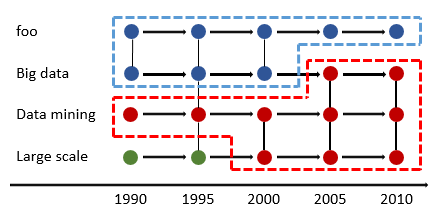
\includegraphics[width=0.80\linewidth]{figures/mutual.png}
\end{center}

\begin{itemize}

\item \textbf{Representativeness:} 
To capture the semantic relationship between terms, we connect terms co-occurred in the documents at the same time slide with representative edges. Formally, the weight of the directed edge $(n_i^t,n_j^t)$ is defined based on mutual information, indicates how appropriate it is to use term $w_i$ to represent $w_j$ at time $t$. We calculate mutual information between term $w_i$ and term $w_j$ at the given time slide $t$ as:
\begin{equation}
\begin{split}
I(n_i^t,n_j^t) & = p(w_i \in d_t, w_j \in d_t)log{\frac{p(w_i\in d_t, w_j \in d_t)}{p(w_i \in d_t)p(w_j \in d_t)}} \\
& + p(w_i \in d_t, w_j \notin d_t)log{\frac{p(w_i\in d_t, w_j \notin d_t)}{p(w_i \in d_t)p(w_j \notin d_t)}} \\
& + p(w_i \notin d_t, w_j \in d_t)log{\frac{p(w_i\notin d_t, w_j \in d_t)}{p(w_i \notin d_t)p(w_j \in d_t)}} \\
& + p(w_i \notin d_t, w_j \notin d_t)log{\frac{p(w_i\notin d_t, w_j \notin d_t)}{p(w_i \notin d_t)p(w_j \notin d_t)}}
\end{split}
\end{equation}

where $d_t$ denotes all the retrieved documents at time $t$. The representativeness of term $w_i$ to term $w_j$ at time $t$ is then defined as normalized mutual information $$s(n_i^t,n_j^t) = \frac{I(n_i^t,n_j^t)}{I(n_i^t,I_i^t)}$$


\item \textbf{Meaning shift:}
Nodes corresponding to the term $w_i$ within two adjacent time slides $-1t$ and $t$ are connected by an evolving edge $(n_i^{t-1},n_i^{t})$, indicates that the term is evolved from itself at the last time slide. The weight of the evolving edge indicates whether the meaning of the term is staying the same or shifted from time $t-1$ to $t$. Formally the weight is defined based on Jaccard coeffient.
$$s(n_i^{t-1},n_i^t) = \frac{|NB(n_i^{t-1}) \cap NB(n_i^t)|}{|NB(n_i^{t-1}) \cup NB(n_i^t)|}$$

\item \textbf{Burstiness:}
We model burstiness by assuming the arrival of terms as an unknown binomial distribution, and use $\chi^2$ tests to check for significant association between words and time periods. We calculate the contingency table as below and $\chi^2 = \frac{(ad-bc)^2n}{(a+b)(c+d)(a+c)(b+d)}$.
\begin{center}
\begin{tabularx}{0.5\linewidth}{ |X|X|X| }
  \hline
  - & $W$ & $\bar{W}$ \\
  \hline
  $t$  & a  & b  \\
  \hline
  $<t$  & c  & d  \\
  \hline
\end{tabularx}
\end{center}

We define burstiness of term $w_i$ at time $t$ as $b_i^t = \chi^2$ value.

\item \textbf{Authority:}
We simply defined the authority of a term at a given time by $u_i^t=df_t(w_i)/|d_t|$, where $df_t(w_i)$ indicates the document frequency of $w_i$ at time $t$, and $|d_t|$ is the number of documents at time $t$.
\end{itemize}




\subsection{Trend Partitioning}
In order to give a concise and intuitive summarization, we need to partition the dynamic concept graph into evolutionary trends, and select a set of representative terms best describe the development of the research topic. Here, we use a massage passing algorithm to perform the selection and partition. The method is analogous to affinity propagation(AP) algorithm proposed in Frey et al. and Tang et al, the difference is that our method is modified to fit the dynamic setting. The AP algorithm performs clustering by identifying exemplars. Essentially it solves the following optimization problem
$$c^* = argmin(-\sum S(i,c_i) )$$
where $C=(c_i)$ is the mapping between nodes and exemplars, $S(i,c_i)$ indicates the similarity between $i$ and its exemplar. $S(i,i)$ is the penalty for i to being exemplar of itself.

In the algorithm, we introduce three sets of variables $\{r_{ij}^t\}$, $\{a_{ij}^t\}$ and $\{e_i^{t-1,t}\}$. Where $r_{ij}^t$ indicates the how well-suited term $w_j$ is to serve as an exemplar of term $w_i$ (i.e. $w_j$ covers the meaning of $w_i$) at time slide $t$. $a_{ij}$ denotes the availabilities of term $w_j$ to serve as an exemplar of $w_i$ at time $t$. $\{e_i^{t-1,t}\}$ indicates the equivalence between the term $w_i$ at two adjacent time slides which captures to what extent the meaning of term $w_i$ has shifted from $t-1$ to $t$.
All the $r_{ij}^t$, $a_{ij}^t$ and $e_i^{t-1,t}$ are set to $0$ initially, their values are updated iteratively with following rules until convergence.
\beal{
r_{ij}^t = (1-\lambda)\rho_{ij}^t+\lambda r_{ij}^t\\
a_{ij}^t = (1-\lambda)\alpha_{ij}^t+\lambda a_{ij}^t
}
where $\lambda$ is a damping factor, $\rho_{ij}^t$ and $\alpha_{ij}^t$ are messages passing from $n_i^t$ to $n_j^t$. The massage passing rules are defined as follows:


\beal{
\rho_{ij}^t = s(n_i^t,n_j^t) - \max_{k\in NB(n_j^t)}\{s(n_i^t,n_k^t) + a_{ik}^t\}\\
\alpha_{ii}^t = \sum_{k\in NB(n_i^t)}\max\{0,r_{ij}^t\}\\
\alpha_{ij}^t = min\{0,r_{jj}^t + \sum_{k \in NB(n_j^t)}\max\{0,r_{ik}^t\}\}
}

\begin{algorithm}[t]
\label{alg:learning}
\caption{Message passing algorithm on dynamic concept graph.}
\small
% factor graph learning
%Learning step:
%\BlankLine
\SetLine \KwIn{dynamic concept graph $G=\{V,E_r,E_e\}$;}
\KwOut{a set of representative nodes $V_r$ and the par;}
%// Generate train data\;
%$G=\emptyset$\;
Initialize all ${r_{ij}^t}\leftarrow\mathbf{0}$\;
\Repeat{converge}{
    \ForEach{edge ($n_i^t$)}{
     //Initialization\;
    $L \leftarrow$ initialization list\;
    %$inventorction(L)$\;
    %$L \leftarrow RemoveUnlabelNodes(L)$\;

%\BlankLine
Factor graph $FG \leftarrow BuildFactorGraph(L)$\;

// Learn the parameter $\mathbf{\theta}$ for factor graph model\;
%$order \leftarrow BuildUpdateOrder(FG)$\;

\Repeat{(all messages $\mu$ do not change)}{
    \ForEach {$v_i \in order$} {
        Update the messages of $v_i$\ by Eqs.~\ref{eq:sp_v} and \ref{eq:sp_f};
    }
}
\ForEach{$\theta_i\in \mathbf{\theta}$} {
    Calculate gradient $\nabla_i$ according to Eq. \ref{eq:gradient}\;
    Update $\theta^{new} = \theta^{old} + \eta \cdot \nabla_i$\;
}
}
}
\normalsize
\end{algorithm}

where $NB(n_j^t)$ denotes the neighboring nodes of node $n_j^t$, $s(n_i^t,n_j^t)$ is $w_i$'s representativeness of $w_j$ at time $t$. $s(n_i^t,n_i^t)$ is set to $s(n_i^t,n_i^t) = \beta b_i^t + (1-\beta)u_i^t$ indicates that the nodes with high authority and burstiness are preferred to be choose as exemplars, where $\beta$ is a parameter controlling the trade-off between timeliness and importance. 



